\documentclass[14pt]{beamer}
\usetheme{Dresden}
\usecolortheme{orchid}

\usepackage{xcolor}
\usepackage{listings}
\usepackage{courier}
\usepackage{graphicx}
\usepackage{amsmath}
\usepackage{algorithm2e}
\usepackage{multicol}
\usepackage{amssymb}

\usefonttheme[onlymath]{serif}

\definecolor{mGreen}{rgb}{0,0.6,0}
\definecolor{mGray}{rgb}{0.5,0.5,0.5}
\definecolor{mPurple}{rgb}{0.8,0,0.82}
\definecolor{backgroundColour}{rgb}{0.95,0.95,0.92}
\definecolor{lightBlue}{rgb}{0.1, 0.1, 0.8}

\lstdefinestyle{CStyle}{
    backgroundcolor=\color{backgroundColour},   
    commentstyle=\color{mGreen},
    keywordstyle=\color{magenta},
    numberstyle=\tiny\color{mGray},
    stringstyle=\color{mPurple},
    basicstyle=\footnotesize\ttfamily,
    breakatwhitespace=false,         
    breaklines=true,                 
    captionpos=b,                    
    keepspaces=true,                 
    numbers=left,                    
    numbersep=5pt,                  
    showspaces=false,                
    showstringspaces=false,
    showtabs=false,                  
    tabsize=2,
    language=C
}

\lstdefinestyle{Ctable}{
    backgroundcolor=\color{backgroundColour},   
    commentstyle=\color{mGreen},
    keywordstyle=\color{magenta},
    numberstyle=\tiny\color{mGray},
    stringstyle=\color{mPurple},
    basicstyle=\footnotesize\ttfamily,
    breakatwhitespace=false,         
    breaklines=true,                 
    captionpos=b,                    
    keepspaces=true,                                  
    showspaces=false,                
    showstringspaces=false,
    showtabs=false,                  
    tabsize=2,
    language=C
}

\lstdefinestyle{pseudo}{
        basicstyle=\ttfamily\footnotesize,
        keywordstyle=\color{lightBlue},
        morekeywords={BEGIN,END,IF,ELSE,ENDIF,ELSEIF,PRINT,WHILE,RETURN,ENDWHILE,DO,FOR,TO,IN,ENDFOR,BREAK,INPUT,READ},
        morecomment=[l]{//},
        commentstyle=\color{mGreen}
}

\lstset{basicstyle=\footnotesize\ttfamily,breaklines=true}
\lstset{framextopmargin=50pt,tabsize=2}

\title{ENGG1003 - Monday Week 5}
\subtitle{Static Variables\\Commenting\\Arrays\\Maybe Strings}
\author{Brenton Schulz}
\institute{University of Newcastle}
\date{\today}


\begin{document}
\titlepage

\begin{frame}[fragile]
\frametitle{Static Variable Example}
\begin{itemize}
\item Example: Write a function, \texttt{counter()} which returns an integer equal to the number of times it has been called.
\pause
\item Function prototype: \texttt{int counter(void);}
\pause
\item Function definition:
\begin{lstlisting}[style=CStyle]
int counter() {
	static int count = 0;
	return count++;
}
\end{lstlisting}
\end{itemize}
\end{frame}

\begin{frame}[fragile]
\frametitle{Static Variable Example}
\begin{itemize}
\item The variable \texttt{count} is declared \texttt{static}
\item The initialisation, \texttt{count = 0}, happens \textit{once}
\item The value of \texttt{count} is retained between function calls 
\begin{lstlisting}[style=CStyle]
int counter() {
	static int count = 0;
	return ++count;
}
\end{lstlisting}
\end{itemize}
\end{frame}

\begin{frame}
\frametitle{Static Variable Example}
\begin{itemize}
\item Wait, why would you do this?
\pause
\item The function can be called from \textit{anywhere} in your code
\pause
\item A ``counter'' variable that did the same job would have to be ``global'' to be visible anywhere
	\begin{itemize}
\pause
		\item For multiple reasons we try to avoid variables with global scope
			\begin{itemize}
				\item Good discussion \underline{\href{http://wiki.c2.com/?GlobalVariablesAreBad}{here}}
			\end{itemize}
\pause
		\item There are \textit{very good} reasons to use them in embedded systems, but not on a desktop PC or server
	\end{itemize}
\end{itemize}
\end{frame}

\begin{frame}[fragile]
\frametitle{Static Variable Example}
Wrapping the function in some test code:
\begin{lstlisting}[style=CStyle]
#include <stdio.h>

int counter(void);

int main() {
	for(int k = 0; k < 10; k++)
		printf("counter(): %d\n", counter() );
	return 0;
}

int counter(void) {
	static int count = 0;
	return count++;
}
\end{lstlisting}
\end{frame}

\begin{frame}
\frametitle{Test Code?}
\begin{itemize}
\item ``Test code'' is a term I made up
\item It means the minimum amount of code required to verify a function's behaviour
\item Always test your functions \textit{in isolation}!
\pause
\item If you write ``too much'' code before testing it will make debugging \textbf{much} harder
\end{itemize}
\end{frame}

\begin{frame}
\frametitle{Test Code}
\begin{itemize}
\item How much is ``too much''?
\pause
\item Personally?
\pause
\item After 20 years of experience?
\pause
	\begin{itemize}
		\item 1-5 lines
	\end{itemize}
\pause
\item Never underestimate:
	\begin{itemize}
		\item How hard programming is
		\item How easy it is to make mistakes
		\item How \textit{brutally catastrophic} bugs can be
	\end{itemize}
\end{itemize}
\end{frame}

\begin{frame}
\frametitle{Bug Case Study}
Paraphrased from \underline{\href{https://en.wikipedia.org/wiki/Therac-25}{Wikipedia}}:
\\~\\
``The Therac-25 was a computer-controlled radiation therapy machine ... It was involved in at least six accidents ...  in which patients were given massive overdoses of radiation. Because of concurrent programming errors, it sometimes gave its patients radiation doses that were hundreds of times greater than normal, resulting in death or serious injury.''
\end{frame}

\begin{frame}
\frametitle{Back to Functions...}
\begin{itemize}
\item When should functions be used?
\pause
\item Well, what do they achieve?
	\begin{itemize}
		\item \textit{Much} easier to solve problems when they're broken down into sub-tasks
		\item Reduce code line count and complexity (if they are called multiple times)
		\item Allows code re-use between projects
		\item \textit{Much} easier to perform project management between multiple programmers
		\item Bugs in a function are easier to fix than a bug in code which has been copy+pasted multiple times
		\item ...the list goes on
	\end{itemize}
\end{itemize}
\end{frame}

\begin{frame}
\frametitle{When should functions be used?}
\begin{itemize}
\item What about in an ENGG1003 context?
\pause
	\begin{itemize}
		\item Vague rule of thumb? No more 10-20 lines or so in one block.
		\item Break a big problem into multiple sub-problems
			\begin{itemize}
				\item Implement each as their own function
				\pause
				\item Yes, even if they are only called once
				\pause
				\item Do what you feel is most ``readable''
				\pause
				\item Your opinion here will change with experience, I will try to provide guidance
			\end{itemize}
	\end{itemize}
\end{itemize}
\end{frame}

\begin{frame}[fragile]
\frametitle{Indenting}
\begin{itemize}
\item At the request of multiple demonstrators, lets talk about code indentation
\pause
\item This one sparks joy:
\begin{lstlisting}[style=CStyle]
main() {
	int x;
	// do stuff
	if(x < 0) {
		// do other stuff
		x++;
	}
}
\end{lstlisting}
\end{itemize}
\end{frame}

\begin{frame}[fragile]
\frametitle{Indenting}
\begin{itemize}
\item This one does not spark joy:
\begin{lstlisting}[style=CStyle]
main() {
int x;
// do stuff
if(x < 0) {
// do other stuff
x++;
}
}
\end{lstlisting}
\end{itemize}
\end{frame}

\begin{frame}[fragile]
\frametitle{Indenting}
\begin{itemize}
\item My eyes! The goggles do nothing!
\begin{lstlisting}[style=CStyle]
main() { int x; // do stuff
if(x < 0) { /* do other stuff */ x++; }}
\end{lstlisting}
\pause
\item We indent to make code easier to read
\item Every block gets indented by one tab 
	\begin{itemize}
		\item Or 2-4 spaces
	\end{itemize}
\item Try to keep one statement per line
\end{itemize}
\end{frame}

\begin{frame}[fragile]
\frametitle{Indenting}
\begin{itemize}
\item Lots of indentation styles exist
\item Indentation is the correct word
	\begin{itemize}
		\item I say indenting because I'm slack
	\end{itemize}
\item Great list on \underline{\href{https://en.wikipedia.org/wiki/Indentation_style}{Wikipedia}}
\item In industry, different companies / teams / projects can use different indentation styles
	\begin{itemize}
		\item None of them are ``better'' than the others
		\item The ``best'' is ``whatever you're used to''
		\item I vaguely follow ``K\&R'' style
	\end{itemize}
\pause
\item Pick a style you like and \textit{be consistent}
\end{itemize}
\end{frame}

\begin{frame}
\frametitle{Functions and Comments}
\begin{itemize}
\item Programming courses always tell you to comment your code
\item But what is ``good'' commenting?
\item Lets look at some examples:
\pause
	\begin{itemize}
		\item From the \underline{\href{https://raw.githubusercontent.com/torvalds/linux/master/kernel/async.c}{Linux kernel source}}
		\pause
		\item From an \underline{\href{http://libopencm3.org/docs/latest/stm32f4/html/adc_8c_source.html}{embedded systems library}}
	\end{itemize}
\pause
\item Just a little different from each other, eh?
\item Commenting is very application specific
\item Commenting is very audience specific
\end{itemize}
\end{frame}

\begin{frame}
\frametitle{Commenting in ENGG1003}
\begin{itemize}
\item How many comments do we use in ENGG1003?
\item On one hand: only comment what \textit{you} need
\item On the other: we need to assess your comments eventually...
\pause
\item And the assessment needs to minimise demonstrator judgement...
\pause
\item Maybe I create different strict rules for different assignments? Similar to ENGG1500 report rules.
\end{itemize}
\end{frame}

\begin{frame}
\frametitle{Arrays}
\begin{itemize}
\item Anyway, new topic!
\item So far: all variables have been a \textit{single} number
\item What do you do if you need a million of them?
\pause
\item Declare a million variables?
\pause
\item Cry?
\pause
\item Use an \textit{array}!
\pause
	\begin{itemize}
		\item Maybe still cry...at first.
	\end{itemize}
\pause
\item An \textit{array} is a collection of variables of the same data type
\end{itemize}
\end{frame}

\begin{frame}
\frametitle{Arrays}
\begin{itemize}
\item Remember the mathematics notation:
\begin{equation*}
x_0, x_1, x_2, x_3, ...
\end{equation*}
\item We used it for a single variable, $x$, changing with time
	\begin{itemize}
		\item The ``old'' values of $x$ were discarded
	\end{itemize}
\pause
\item An array allows us to store \textit{all} the values of $x_n$ in memory
\item The variable name, $x$, and the ``index'', $n$, are both needed to access a particular value
\end{itemize}
\end{frame}

\begin{frame}
\frametitle{Arrays}
\begin{itemize}
\item In C, an array declaration \textbf{needs} three things:
	\begin{itemize}
		\item The data type
		\item A name
		\item The number of \textit{elements}
	\end{itemize}
\item (Optional) Arrays can be initialised
\item The syntax for an array of length N is:\\
\texttt{data\_type name[N];}
\item Examples:
	\begin{itemize}
		\item \texttt{int list[20];}
		\item \texttt{char name[200], c; //array and var}
		\item \texttt{double data[100000];}
	\end{itemize}
\end{itemize}
\end{frame}

\begin{frame}[fragile]
\frametitle{Arrays}
\begin{itemize}
\item The length may be a variable
	\begin{itemize}
		\item Careful: ``a'' variable, lengths don't change
	\end{itemize}
\item The variable's value must be known at the time of declaration
\item \underline{\href{https://i.kym-cdn.com/photos/images/newsfeed/001/401/347/312.jpg}{This is fine}}:
\begin{lstlisting}[style=CStyle]
int x;
scanf("%d", &x);
int array[x];
\end{lstlisting}
\pause
\begin{itemize}
\item If \texttt{x} is large enough your program will access memory the operating system has not allowed it to
\pause
\item This will cause segmentation faults (Linux/macOS) or illegal operations (Windows)
\end{itemize}
\end{itemize}
\end{frame}

\begin{frame}[fragile]
\frametitle{Using Arrays}
\begin{itemize}
\item A C array of size $N$ is \textit{indexed} from $0$ to $N-1$
	\begin{itemize}
		\item Programmers get \textit{illogically angry} when arguing about 0-indexing Vs 1-indexing
	\end{itemize}
\item To access an \textit{element} use the syntax:\\
\begin{lstlisting}[style=CStyle]
arrayName[index]
\end{lstlisting}
where \texttt{index} \textbf{must be an integer}
\item Each array index has a \textit{different} physical memory address
\item Each array index accesses a unique variable
\end{itemize}
\end{frame}

\begin{frame}[fragile]
\frametitle{Array Initialisation}
\begin{itemize}
\item General rule: all variables need to be initialised before use
\item For arrays, there are two solutions:
	\begin{enumerate}
		\item Initialise at declaration with the syntax:
		\begin{lstlisting}[style=CStyle]
int x[10] = {1,2,3,4,5,6,7,8,9,0};
\end{lstlisting}
		When doing this the size is optional:
		\begin{lstlisting}[style=CStyle]
int x[] = {1,2,3}; // int x[3]
\end{lstlisting}
		\item Manually initialise in a loop
	\end{enumerate}
\end{itemize}
\end{frame}

\begin{frame}[fragile]
\frametitle{Array Initialisation}
\begin{itemize}
\item When the array is ``large'' do this instead:
\begin{lstlisting}[style=CStyle]
int x[N];
int counter;
for(counter = 0; counter < N; counter++) {
	x[counter] = 0;
}
\end{lstlisting}
\end{itemize}
\end{frame}

\begin{frame}[fragile]
\frametitle{Array Usage}
\begin{itemize}
\item Array elements can be used anywhere that variables, literals, and function return values can be used
\item This includes:
	\begin{itemize}
		\item In arithmetic expressions
		\item As function arguments
		\item As lvalues (left side of \texttt{=})
	\end{itemize}
\item Examples:
	\begin{itemize}
		\item \texttt{x = y[12] + 28.0;}
		\item \texttt{x[0] = 1.0;}
		\item \texttt{printf("\%f\textbackslash n", x[2]);}
		\item \texttt{y = sin(x[i]);}
	\end{itemize}
\end{itemize}
\end{frame}

\begin{frame}[fragile]
\frametitle{Array Usage}
\begin{itemize}
\item Arrays are very frequently used in loops
\item Example: add up all numbers in an array:
\begin{lstlisting}[style=CStyle]
float x[1000];
// x[] gets filled with numbers somehow
float sum = 0;
float i; // Array index
for(i = 0; i < 1000; i++)
	sum = sum + x[i];
\end{lstlisting}
\pause
\item The Week 5 lab gets you to use an array in statistical analysis
\end{itemize}
\end{frame}

\begin{frame}
\frametitle{When to use Arrays}
\begin{itemize}
\item An array must be used when a loop is used to process data
	\begin{itemize}
		\item There is no other way to ``index'' individual variables
	\end{itemize}
\item Arrays are required to process \textit{strings}
	\begin{itemize}
		\item Written ASCII text, seen later
	\end{itemize}
\item An array \textit{should} be used when it is a convenient way to group together multiple variables with a similar ``theme''
	\begin{itemize}
		\item This is for readability and maintainability
	\end{itemize}
\end{itemize}
\end{frame}

\begin{frame}[fragile]
\frametitle{Array Problems}
\begin{itemize}
\item The size of an array is not intrinsically known
\item You must manually make sure that the array index never exceeds the array's boundary!
\item The following program is \textbf{guaranteed} to crash:
\begin{lstlisting}[style=CStyle]
#include <stdio.h>

int main() {
	int x[10];
	int idx;
	for(idx = 0; idx < 100000000000L; idx++)
		printf("%d\n", x[idx]);
}
\end{lstlisting}
\end{itemize}
\end{frame}

\begin{frame}
\frametitle{Variables in Memory}
\begin{itemize}
\item Visualising how data fits in computer memory is crucial
\item Foundation principles:
	\begin{itemize}
		\item Everything is stored in binary
		\item Memory locations have \textit{addresses}
		\item Memory is \textit{byte-addressed}
		\item C data types can be multiple bytes long
		\item Variables get unique memory addresses
	\end{itemize}

\end{itemize}
\end{frame}

\begin{frame}
\frametitle{Variables in Memory}
\begin{itemize}
\item Each variable gets a unique ``chunk'' of memory
\item Details are complicated, just imagine they get packed next to each other for now
\item An array is packed into a \textit{contiguous block}
	\begin{itemize}
		\item They are all in single blob, no gaps
		\item \texttt{x[0]} gets the lowest memory address
		\item \texttt{x[1]} the one above that, etc
	\end{itemize}
\item Lets draw some boxes...
\end{itemize}
\end{frame}

\begin{frame}[fragile]
\frametitle{Variables in Memory}
\begin{itemize}
\item How are these variables ``packed'' into memory?
\begin{lstlisting}[style=CStyle]
char a; // 1 byte
int i; // 4 bytes
int x[2]; // 2 integers, each 4 bytes
\end{lstlisting}
\pause
\item What would memory \texttt{x[2]} access?
\pause
\item Each box below is one byte:
\end{itemize}
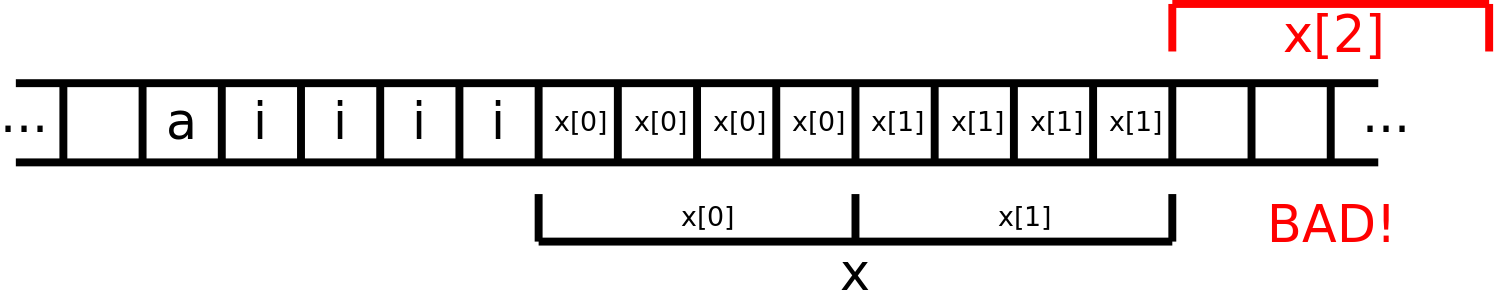
\includegraphics[width=\textwidth]{memory}
\end{frame}

\begin{frame}
\frametitle{Variables in Memory}
\begin{itemize}
\item In that example, \texttt{x[2]} accesses memory outside that allocated to \texttt{x[]}
\item The compiler won't stop you accessing ``bad'' memory addresses!
\item You will either be given ``junk'' data or cause a crash
\item Drawing memory diagrams will help you understand pointers later
\end{itemize}
\end{frame}

\begin{frame}[fragile]
\frametitle{Variables in Memory}
\begin{itemize}
\item Lets study this with a real example
\item The \texttt{\&} symbol is an \textit{operator} which turns a variable name into a memory address
\item We can use this to explore how the compiler allocates memory to variables
\begin{lstlisting}[style=CStyle]
char a; 
int i; 
int x[2]; 
printf("Address of a:   \t%lu\n", &a); 
printf("Address of i:   \t%lu\n", &i); 
printf("Address of x[0]:\t%lu\n", &x[0]); 
printf("Address of x[1]:\t%lu\n", &x[1]); 
\end{lstlisting}
\end{itemize}
\end{frame}

\begin{frame}[fragile]
\frametitle{Variables in Memory}
\begin{itemize}
\item The output on a 64-bit Linux system is:
\begin{lstlisting}[style=pseudo]
Address of a:   	140722511065979
Address of i:   	140722511065980
Address of x[0]:	140722511065984
Address of x[1]:	140722511065988
\end{lstlisting}
\end{itemize}
\end{frame}

\end{document}
